\documentclass{article}

\usepackage{amsmath, amssymb}
\usepackage{tikz}
%\usepackage[margin=1.2in]{geometry}

\newcommand{\pder}[2]{\frac{\partial #1}{\partial #2}}
\newcommand{\pdbder}[2]{\frac{\partial^2 #1}{\partial #2^2}}

\title{
	Loss function for a Poisson 2D inverse problem \\
	of finding a constant unknown forcing
	}

\author{Rajarshi Dasgupta}

\begin{document}

\maketitle

\section{The Problem}

Find the function $u: \Omega \rightarrow \mathbb{R}$
and constant $f$ such that
\begin{align*}
	& - \nabla^2 u(x,y) = f & \mbox{ for } (x,y) \mbox{ in } \Omega \\
	& u(x,y) = 0.3(1 - x^2 - y^2) & \mbox{ for } (x,y) \mbox{ on } \partial \Omega \\
	& u(x_d,y_d) = 0.3(1 - x_d^2 - y_d^2)
\end{align*}
where $\Omega = (-1,1) \times (-1,1)$
and $(x_d,y_d)$ is an internal data point in $\Omega$.
The solution for this problem is
\begin{align*}
	u & = 0.3(1 - x^2 - y^2) \\
	f &= 1.2
\end{align*}
We wish to solve this class of inverse problems
in the FEM framework using ML techniques.

\section{The loss function}

We will be working with a 3 node triangular mesh
over the domain $\Omega$.
The input for the loss function would be
\begin{enumerate}
	\item the vector $u_{\mathit{out}}$
		where the indices are the value of $u$ at each node,
		which would be the output of a GCN,
	\item $f_{\mathit{val}}$, a guess for the unknown constant $f$,
		which would be a trainable parameter,
	\item the stiffness matrix $K \in \mathbb{R}^{n \times n}$,
	\item data forcing vector $f_d \in \mathbb{R}^n$,
	\item and forcing vector $f_0 \in \mathbb{R}^n$
		assuming a forcing of unity,
		that is $f=1$.
\end{enumerate}
where $n$ is the degree of freedom,
that is the number of nodes
on which the value of $u$ is unknown.
If we have a $N \times N$ total nodes,
$n = N^2 - 4N + 3$,
as there are $4(N-2) + 4$ boundary data points
and 1 internal data point.

The loss function we consider is the following.
\begin{align*}
	r &= K u_{\mathit{out}} + f_d - f_{\mathit{val}} f_0 \\
	\mathit{Loss} &= \sum_i r_i^2
\end{align*}
The derivation can be found in the following section.

\section{A derivation for the loss function}

Consider the triangular element $T$
as seen in figure \ref{elems}.
Given a point $O(x,y)$ inside the triangle $V_1V_2V_3$,
we define $\xi$ and $\eta$,
the barycentric coordinates.
\begin{align*}
  \xi &= \frac{\text{area}(OV_2V_3)}{\text{area}(V_1V_2V_3)} \\
  \eta &= \frac{\text{area}(OV_1V_3)}{\text{area}(V_1V_2V_3)} \\
\end{align*}
Let the value of the trial function $u(x,y)$
at the vertices $V_1$, $V_2$ and $V_3$
be $u_1$, $u_2$ and $u_3$ respectively.
Similarly,
let the value of the test function $v(x,y)$
at the vertices $V_1$, $V_2$ and $V_3$
be $v_1$, $v_2$ and $v_3$ respectively.
Now, the points inside or on the triangle
are easily parameterised by $\xi$ and $\eta$
in the following manner.
\begin{align}
  x &= N_1 x_1 + N_2 x_2 + N_3 x_3 \label{x}\\
  y &= N_1 y_1 + N_2 y_2 + N_3 y_3 \label{y}
\end{align}
where
\begin{align*}
	N = \begin{bmatrix} N_1 & N_2 & N_3 \end{bmatrix} \\
	N_1, N_2, N_3 = \xi, \eta, 1 - \xi - \eta
\end{align*}

Assuming $V_1$, $V_2$ and $V_3$ to be free nodes,
the finite dimensional weak formulation
for the Poisson's problem in two dimensions
for the triangular element $T$
is to find $\hat{u} = \begin{bmatrix} u_1 & u_2 & u_3 \end{bmatrix}^{\mathsf{T}}$
such that
\begin{align}
	\int_T \pder{v}{x}\pder{u}{x} + \pder{v}{y}\pder{u}{y} dxdy = \int_T fv dxdy \label{weak}
\end{align}
for all $\hat{v} = \begin{bmatrix} v_1 & v_2 & v_3 \end{bmatrix}^{\mathsf{T}}$,
where,
\begin{align*}
	& u(x(\xi,\eta), y(\xi,\eta)) = N \hat{u} \\
	& v(x(\xi,\eta), y(\xi,\eta)) = N \hat{v} \\
\end{align*}
Following standard procedure,
to find algebraic equations for the element,
we start from
\begin{align*}
	\begin{bmatrix} {\partial u}/{\partial \xi} \\ {\partial u}/{\partial \eta} \end{bmatrix}
		& = J \begin{bmatrix} {\partial u}/{\partial x} \\ {\partial u}/{\partial y} \end{bmatrix} 
			& J = \begin{bmatrix} x_1 - x_3 & y_1 - y_3 \\ x_2 - x_3 & y_2 - y_3 \end{bmatrix} \\
	\implies \begin{bmatrix} {\partial u}/{\partial x} \\ {\partial u}/{\partial y} \end{bmatrix}
		& = J^{-1} \begin{bmatrix} {\partial u}/{\partial \xi} \\ {\partial u}/{\partial \eta} \end{bmatrix} \\
		& = J^{-1} \begin{bmatrix} u_1 - u_3 \\ u_2 - u_3 \end{bmatrix}
\end{align*}
Therefore,
\begin{align}
	\begin{bmatrix} {\partial u}/{\partial x} \\ {\partial u}/{\partial y} \end{bmatrix}
		&= B \hat{u} \label{ugrad} \\ 
	\begin{bmatrix} {\partial v}/{\partial x} \\ {\partial v}/{\partial y} \end{bmatrix}
		&= B \hat{v} \label{vgrad} \\ 
\end{align}
where,
\begin{align*}
	B = \frac{1}{\det J} 
	\begin{bmatrix} y_2 - y_3 & y_3 - y_1 \\ x_3 - x_2 & x_1 - x_3 \end{bmatrix}
	\begin{bmatrix} 1 & 0 & -1 \\ 0 & 1 & -1 \end{bmatrix}
\end{align*}
So, the LHS of equation \ref{weak} is the following.
\begin{align*}
	& \int_T (B\hat{v})^{\mathsf{T}} (B\hat{u}) dxdy \\
	=& \hat{v}^{\mathsf{T}} B^{\mathsf{T}}B \hat{u} \int_T dxdy \\
	=& \hat{v}^{\mathsf{T}} K_e \hat{u}
\end{align*}
where,
\begin{align*}
	K_e = \frac{\det J}{2} B^{\mathsf{T}}B
\end{align*}
The RHS of equation \ref{weak} is the following.
\begin{align*}
	& \int_T f \hat{v}^{\mathsf{T}} \begin{bmatrix} N_1 \\ N_2 \\ N_3 \end{bmatrix} \det J d\xi d\eta \\
		= & f \hat{v}^{\mathsf{T}} \hat{f}_0 
\end{align*}
where $ \hat{f}_0 = \det J/6 \begin{bmatrix} 1 & 1 & 1 \end{bmatrix}^{\mathsf{T}}$.

\begin{figure}
\centering
\begin{tikzpicture}[scale=0.8]
  \draw (-1,-1) -- (5,-1) -- (5,5) -- (-1,5) -- (-1,-1) ;
  \draw (1,3) node[left] {$V_1$} -- (3,2) node[below] {$V_2$} -- (4,4) node[right] {$V_3$} -- (1,3) ;
  \draw[->] (0,0) -- (1,0) node[right] {$x$} ;
  \draw[->] (0,0) -- (0,1) node[above] {$y$} ;
\end{tikzpicture}
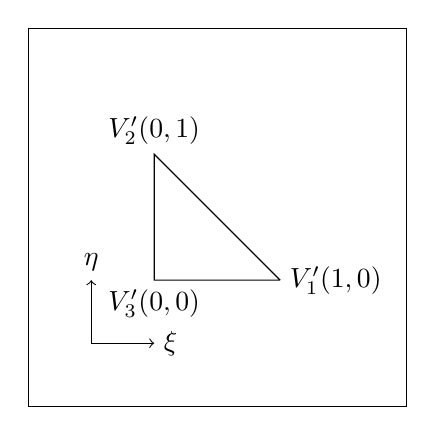
\begin{tikzpicture}[scale=0.8]
  \draw (-1,-1) -- (5,-1) -- (5,5) -- (-1,5) -- (-1,-1) ;
  \draw (3,1) node[right] {$V'_1(1,0)$} -- (1,3) node[above] {$V'_2(0,1)$} -- (1,1) node[below] {$V'_3(0,0)$} -- (3,1) ;
  \draw[->] (0,0) -- (1,0) node[right] {$\xi$} ;
  \draw[->] (0,0) -- (0,1) node[above] {$\eta$} ;
\end{tikzpicture}
\caption{
  The triangular element $T$ in the computaional domain
  is shown on the left
  while its reference element $T'$ 
  is shown on the right.
  }
\label{elems}
\end{figure}

\begin{figure}
\centering
\begin{tikzpicture}[scale=1.8]
  \draw (1,3) node[left] {$V_1$} -- (3,2) node[below] {$V_2$} -- (4,4) node[right] {$V_3$} -- (1,3) ;
  \draw (8/3,3) node[above] {$O$} -- (1,3) ;
  \draw (8/3,3) -- (3,2) ;
  \draw (8/3,3) -- (4,4) ;
  \draw[->] (0,0) -- (1,0) node[right] {$x$} ;
  \draw[->] (0,0) -- (0,1) node[above] {$y$} ;
\end{tikzpicture}
\caption{
  To define parameters $\xi$ and $\eta$
  we form three triangles
  $OV_2V_3$, $OV_3V_1$, and $OV_1V_2$
  which put together form the triangle $V_1V_2V_3$.
  }
\label{bary}
\end{figure}

\end{document}


